% \newcommand\tab[1][0,4cm]{\hspace*{#1}}
\newcommand\longtab[1][1cm]{\hspace*{#1}}
% \setlength{\headheight}{15pt}



\chapter{Generalités sur les applications mobiles}
\section{Introduction}
\tab Dans ces derniers temps, la possession d'un smartphone ou une tablette est devenue indispensable dans notre vie quotidienne, ces derniers sont gérés par de nombreux systèmes d'exploitation.\medskip
\\
Les systèmes d'exploitation sont des logiciels conçus pour faire fonctionner un smartphone en permettant à l'utilisateur de réaliser plusieurs tâches comme passer un appel, prendre des photos et même télécharger des applications pour mieux exploiter son smartphone.\medskip
\\
Dans ce chapitre nous allons nous focaliser sur les différents systèmes d'exploitation et le développement des applications mobiles , nous commençons par une définition d'Android et IOS, ensuite nous allons faire une comparaison entre les deux systèmes d'exploitation et pour finir , nous allons parler sur le développement des applications mobiles et les différents outils utilisés dans ce domaine.\medskip

\section{Les systèmes d'exploitation mobiles}
\subsection{Définition}
Un système d'exploitation mobile est un système d'exploitation conçu pour fonctionner sur un appareil mobile. Ce type de système d'exploitation se concentre entre autres sur la gestion de la connectivité sans fil et celle des différents types d'interface.~\cite{SystemeExploitationMobile}

Les systèmes d'exploitation mobiles sont généralement installés sur les smartphones. Il existe un grand nombre de systèmes d'exploitation tel que : Windows Phone, iOS, Android, BlackberryOs, Symbian OS et Bada.

Les deux systèmes d'exploitation les plus présents en ce temps sont Android de l'entreprise Google et iOS d'Apple. Ces deux systèmes offrent de manière régulière des mises à jour qui améliorent la qualité et les performances du système en plus de renforcement de la sécurité de l'appareil.
 

\subsection{Le système Android}
\begin{wrapfigure}[8]{r}{3cm}
    \vspace{-15pt}
    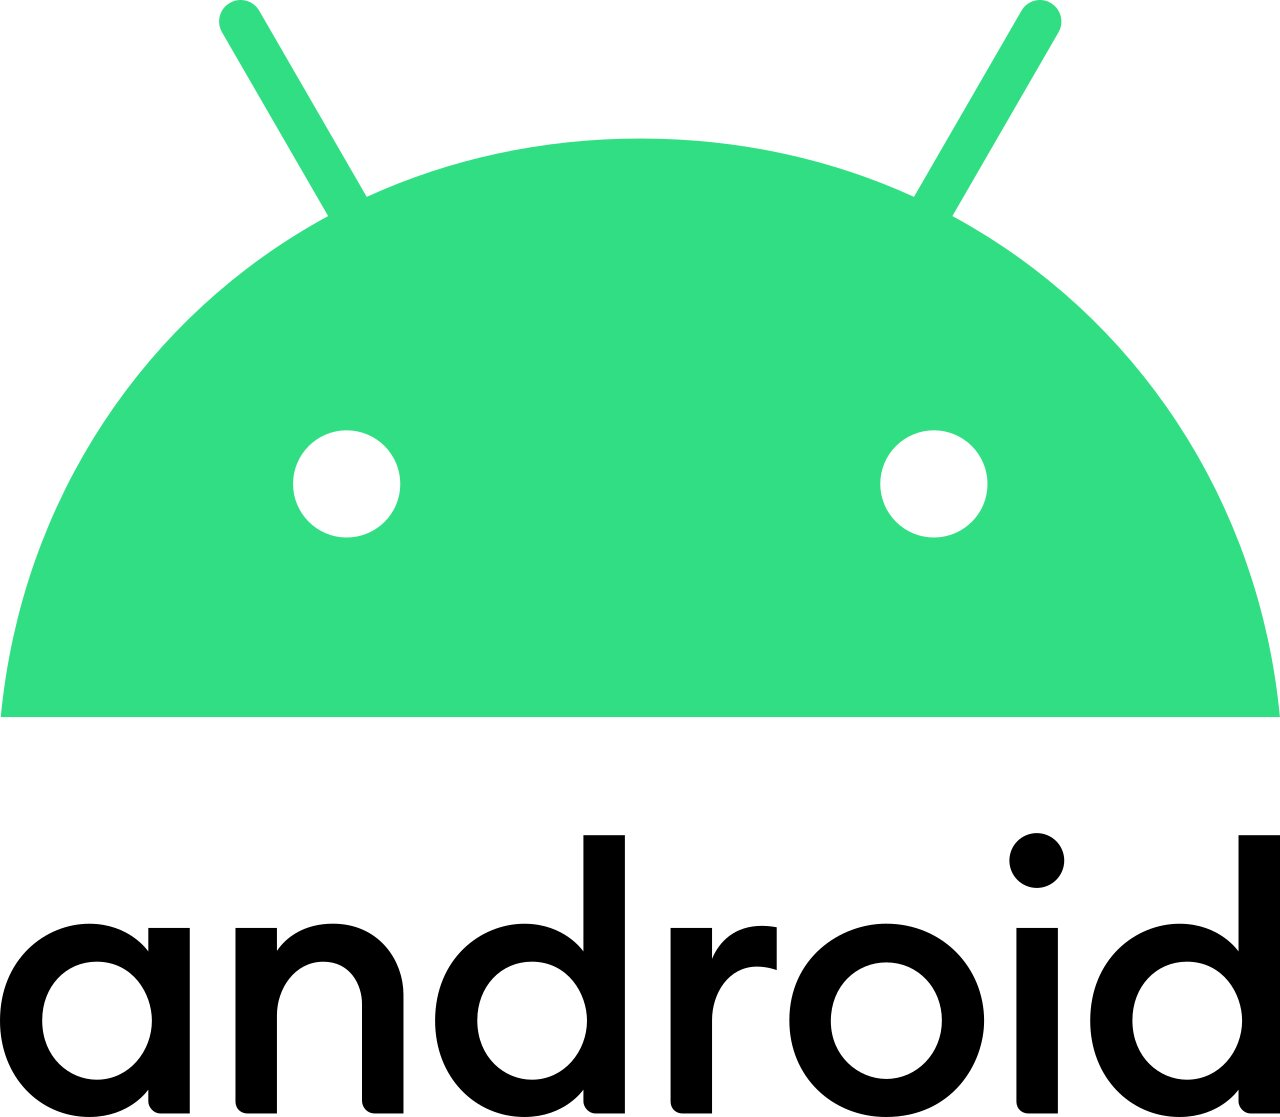
\includegraphics[width=3cm]{images/Chapitre1/android.jpg}
    \vspace{-20pt}
    \caption{{\footnotesize Logo Android}}
\end{wrapfigure}



Android est un système d'exploitation créé par Google, ce système permet d'utiliser son smartphone, le personnaliser et même télécharger des applications pour faciliter les tâches quotidiennes de l'utilisateur et mieux exploiter son appareil.

Lancé en juin 2007 à la suite du rachat par Google en 2005 de la startup du même nom6, le système avait d'abord été conçu pour les smartphones et tablettes tactiles, puis s'est diversifié dans les objets connectés et ordinateurs comme les télévisions (Android TV), les voitures (Android Auto), les Chromebook (Chrome OS qui utilise les applications Android) et les smartwatch (Wear OS).~\cite{AndroidWikipedia}

Le système Android a été développé et ce jusqu'à la version 10 appelée Android Q. Ce système est distribué vers les smartphones et les tablettes sous trois formes : 
\begin{itemize}
    \item Un système d'exploitation customisé en appliquant une surcouche logicielle qui va avec les modèles de chaque constructeur comme One UI de Samsung, MIUI de Xiaomi et EMUI de Huawei. cela apporte une meilleure expérience utilisateur
   
    \begin{figure}[!ht]
        \centering
        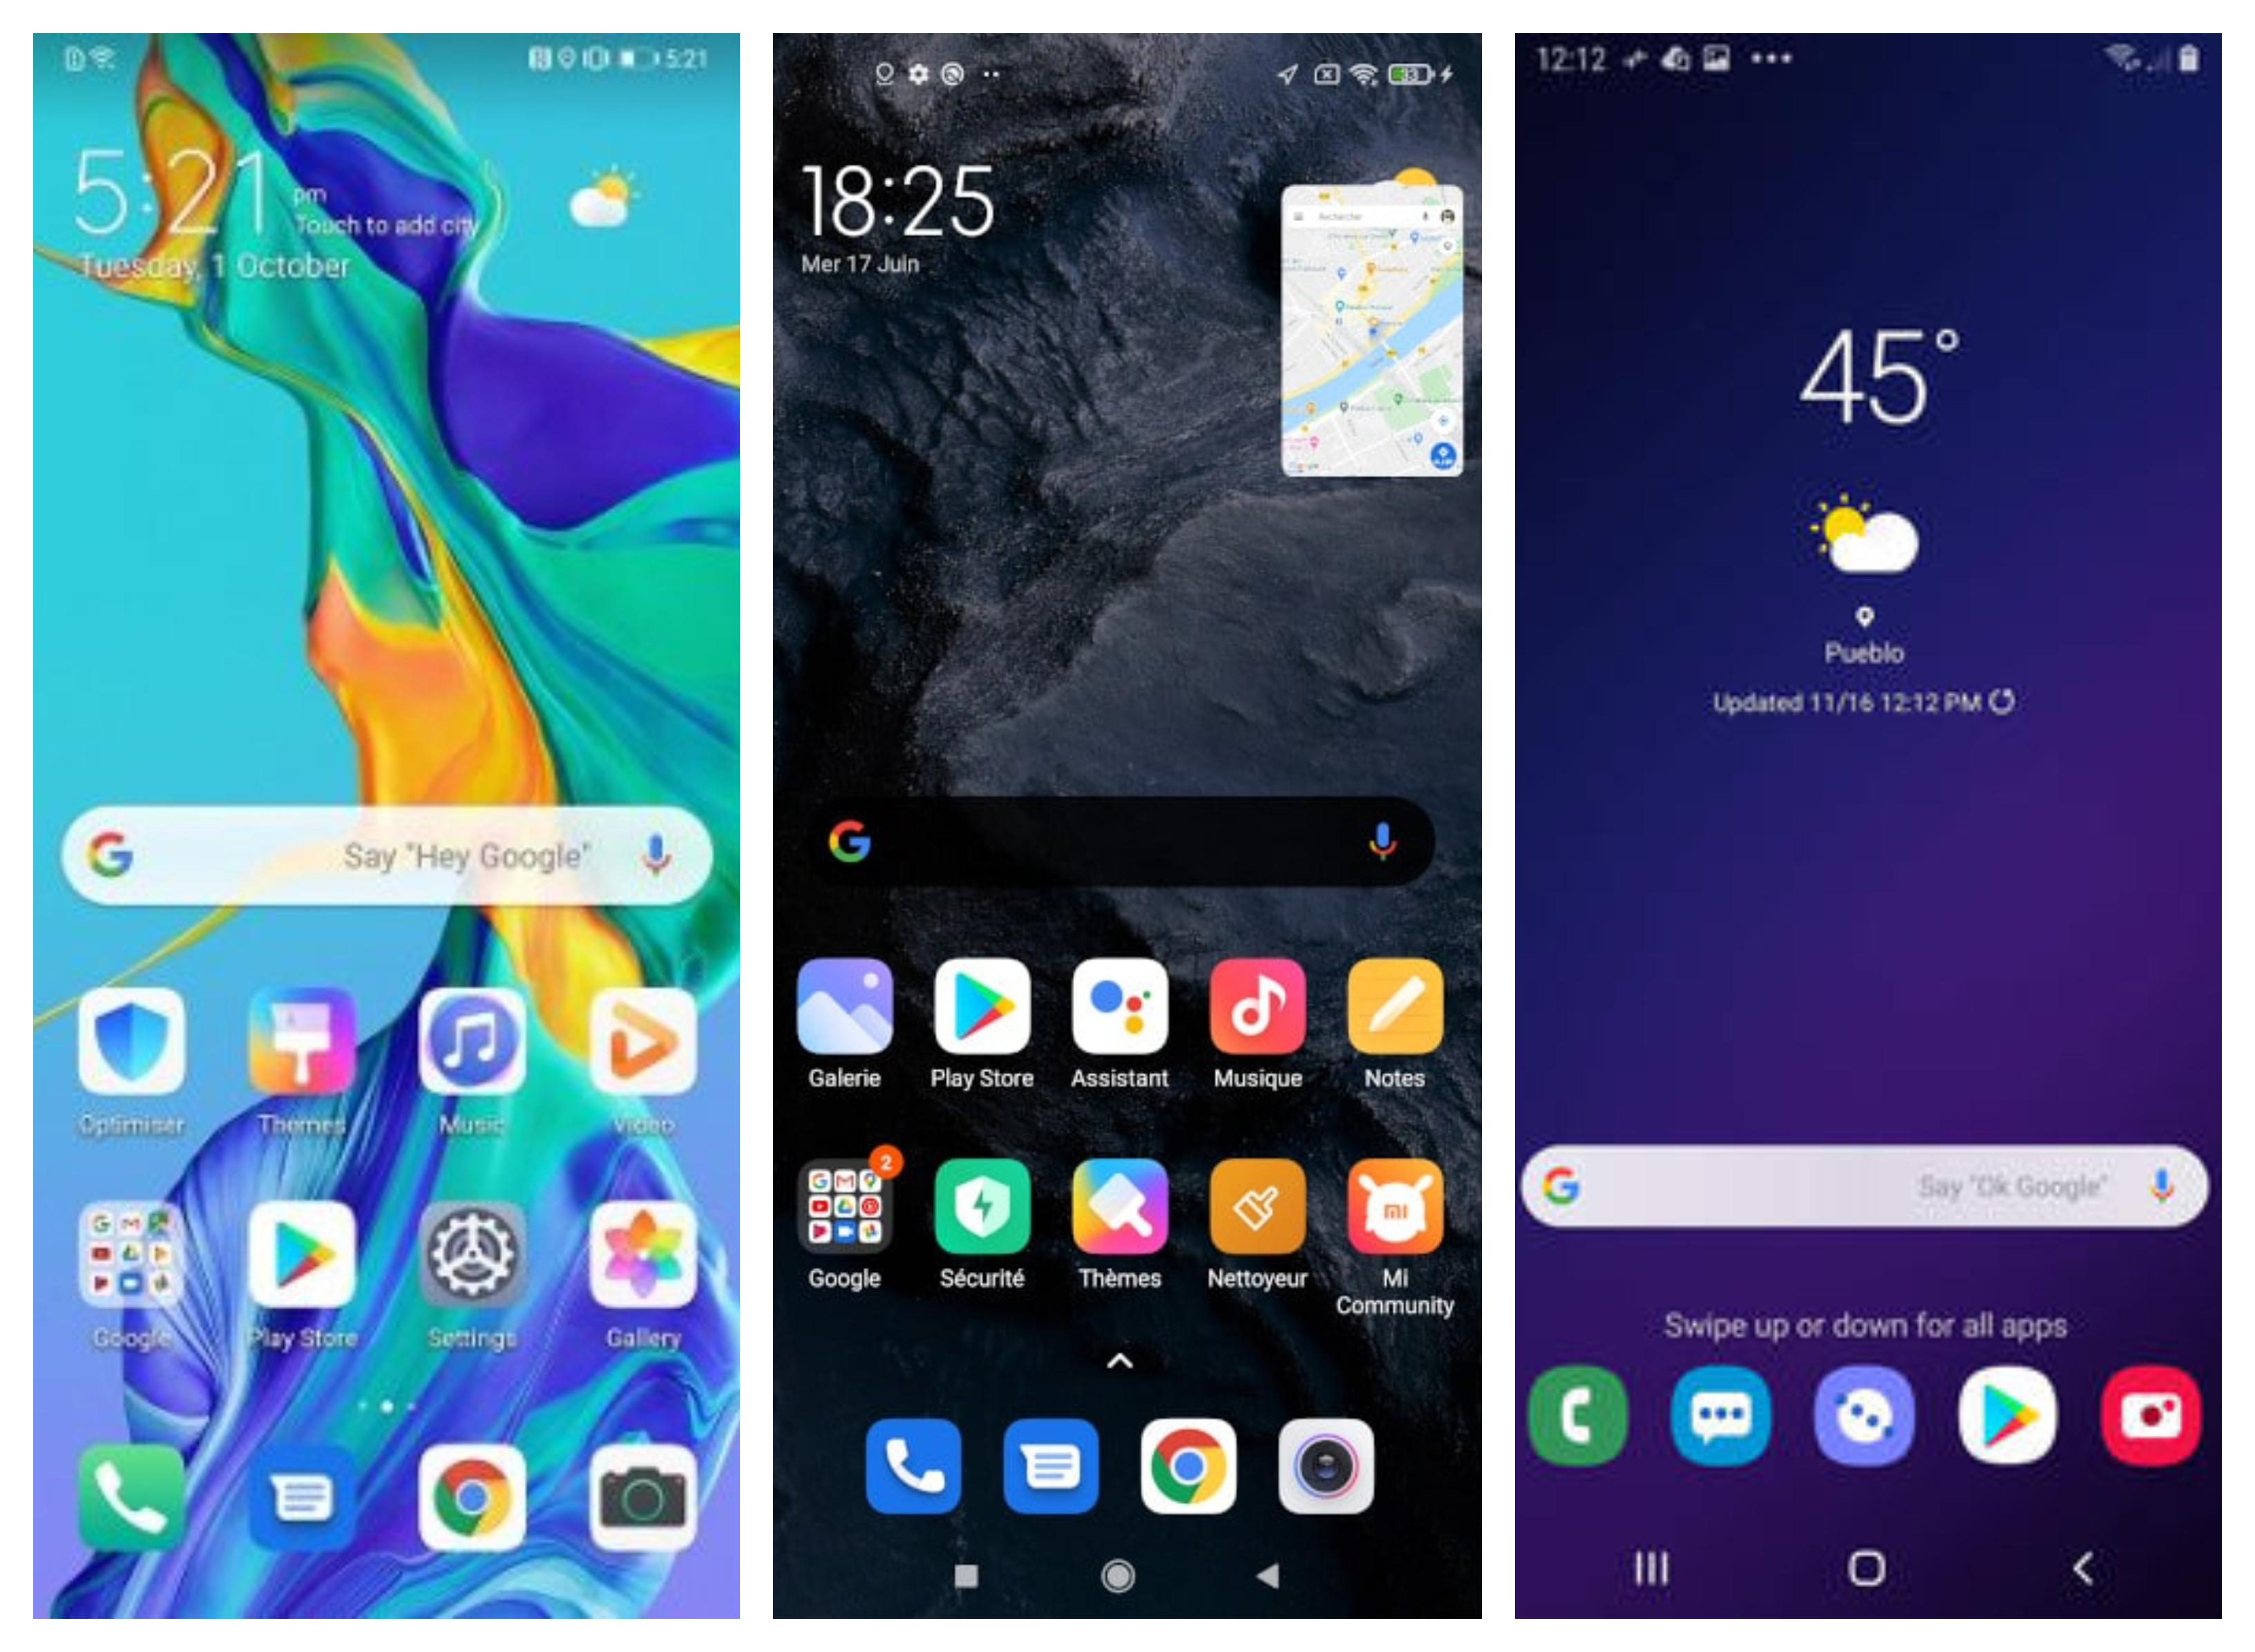
\includegraphics[width=4in]{images/Chapitre1/surcouche.jpg}
        \label{fig:surcouche}
        \caption{Différence entre les surcouches EMUI, MIUI et ONE UI}
    \end{figure}

    \item Un système d'exploitation sans  l'application d'une surcouche. cette version est installé par exemple sur les smartphones Android Go, Ces derniers sont mis à jour rapidement vers de nouvelles versions de ce système.
    \begin{figure}[!ht]
        \centering
        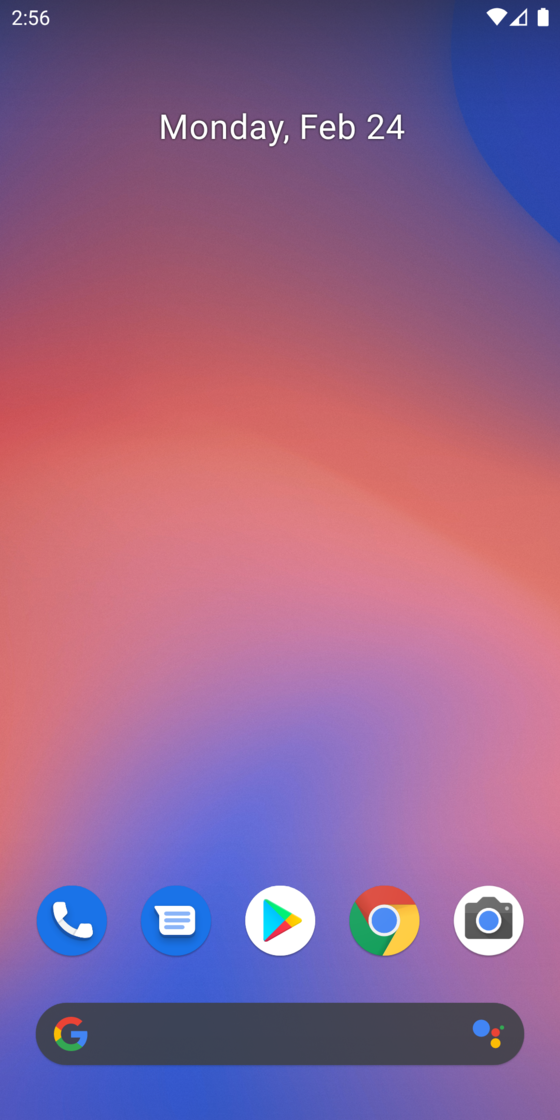
\includegraphics[width=1.5in]{images/Chapitre1/android_R.png}
        \label{fig:androidsanssurcouche}
        \caption{L'interface utilisateur d'Android 10 sans l'application des surcouches}
    \end{figure}
    \item Le système Android est installé aussi sous la forme de versions alternatives appelées Custom ROM. On installe ces ROM par exemple lorsqu'un smartphone est incompatible avec une version Android, ce ROM s'installe avec la version courante d'Android mais avec une interface d'un système différent.
\end{itemize}
\newpage
\tab \textbf{L'architecture d'Android:}\medskip

L'architecture du système Android est sous forme d'une pile de composants comme on le voit dans la figure suivante :
\begin{figure}[!ht]
    \centering
    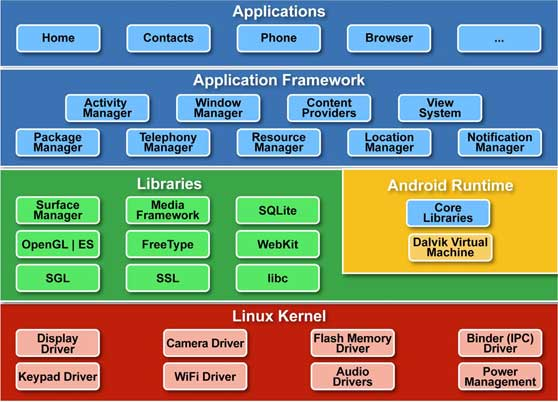
\includegraphics[width=5in]{images/Chapitre1/android_architecture.jpg}
    \label{fig:architecture android}
    \caption{L'architecture d'Android}
\end{figure}

En lisant la figure de bas en haut, on trouve dans la première couche que ce système est basé sur le noyau (ou Kernel) de Linux conçu spécialement pour l'environnement mobile, ce composant joue le rôle d'un pont entre les composants matériels et logiciels. Il contient donc tous les pilotes, ces derniers utilisent des fonctions qui permettent de contrôler le matériel.

Au-dessus du kernel il y a le "Hardware abstraction layer" qui permet de séparer la plateforme logique du matériel. Au-dessus de cette couche d'abstraction on retrouve les librairies C./C++ utilisées par un certain nombre de composants du système Android.
On retrouve ensuite l'Android Runtime, cette couche contient les librairies cœurs du Framework ainsi que la machine virtuelle exécutant les applications. Au-dessus la couche "Android Runtime" et des librairies cœurs on retrouve le Framework permettant au développeur de créer des applications.
Enfin au-dessus du Framework il y a les applications.

\subsection{Le système iOS}
\begin{wrapfigure}[8]{r}{3cm}
    \vspace{-15pt}
    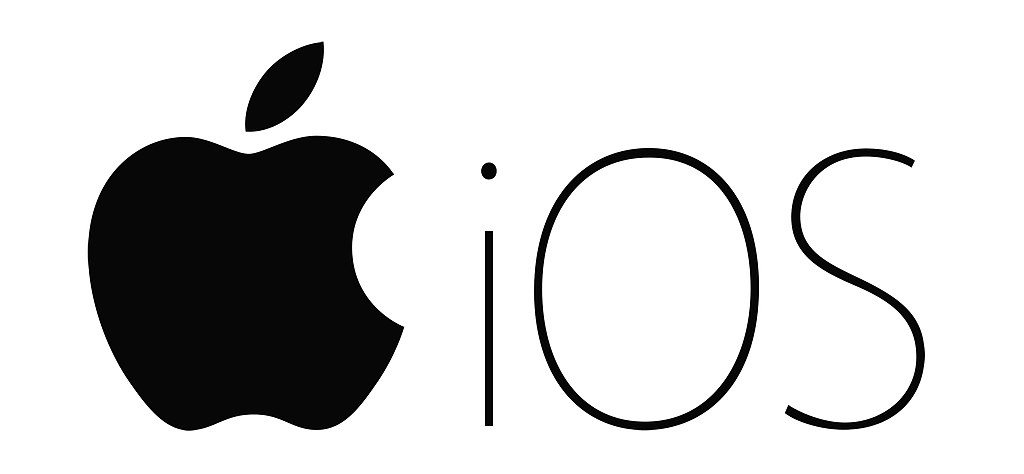
\includegraphics[width=3cm]{images/Chapitre1/ios_logo.jpg}
    \vspace{-20pt}
    \caption{{\footnotesize Logo iOS}}
\end{wrapfigure}

iOS, anciennement iPhone OS , est le système d'exploitation mobile développé par Apple pour plusieurs de ses appareils. Il est dérivé de macOS dont il partage les fondations (le noyau hybride XNU basé sur le micro-noyau Mach, les services Unix et Cocoa, etc.).

iOS comporte quatre couches d'abstraction, similaires à celles de macOS : une couche « Core OS », une couche « Core Services », une couche « Media » et une couche « Cocoa ». Le système d'exploitation occupe au maximum 3 Go de la capacité mémoire totale de l'appareil, selon l'appareil.~\cite{IOS2020}

Ce système d'exploitation est connu par sa rapidité et fluidité sur les appareils d'Apple vu qu'il est développé spécialement pour les iphones contrairement à Android.

\begin{figure}[!ht]
    \centering
    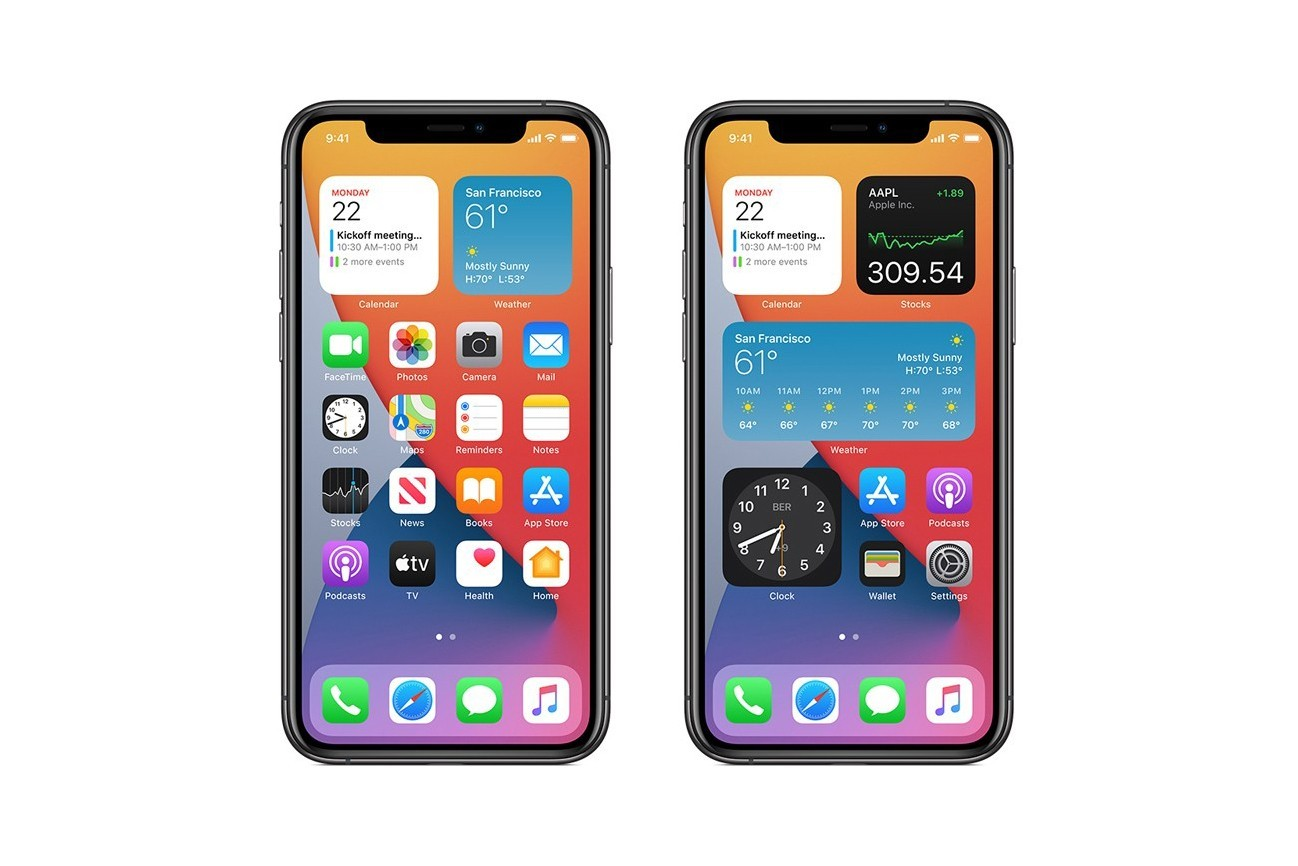
\includegraphics[width=5in]{images/Chapitre1/iosui.jpg}
    \label{fig:ios Ui}
    \caption{L'interface de iOS}
\end{figure}
\newpage
\tab \textbf{L'architecture d'iOS:}\medskip

Comme on l'a déjà mentionné dans la partie précédente, iOS est basé sur macOS. Son architecture est composée de 4 éléments: le BaseBand, le BootLoader,le Firmware et le SeckPack.

\begin{itemize}
    \item Le BaseBand est un micrologiciel autonome qui gère en temps réel tous les périphériques de communication de l'appareil. Le BaseBand est considéré donc comme le BIOS de l'iPhone.
    \item Le BootLoader est le programme chargé du démarrage du système iOS, c'est le premier processus exécuté lorsqu'on allume l'iphone 
    \item Le Firmware est un programme interne dans l'iPhone, ce programme prend contrôle de la partie systématique de l'appareil comme la caméra, l'écran et le clavier tactile. 
    \item Le SeckPack est une partie de la mémoire flash de l'appareil contenant entre autres des informations sur le verrouillage de celui-ci. Le Seckpack peut être considéré comme un mot de passe : en effet, si un SeckPack correct est fourni au BootLoader lors du lancement, alors l'utilisateur a la possibilité d'utiliser le BaseBand, et donc les fonctionnalités de téléphonie et d'Internet.~\cite{IOS2020}
\end{itemize}

\begin{figure}[!ht]
    \centering
    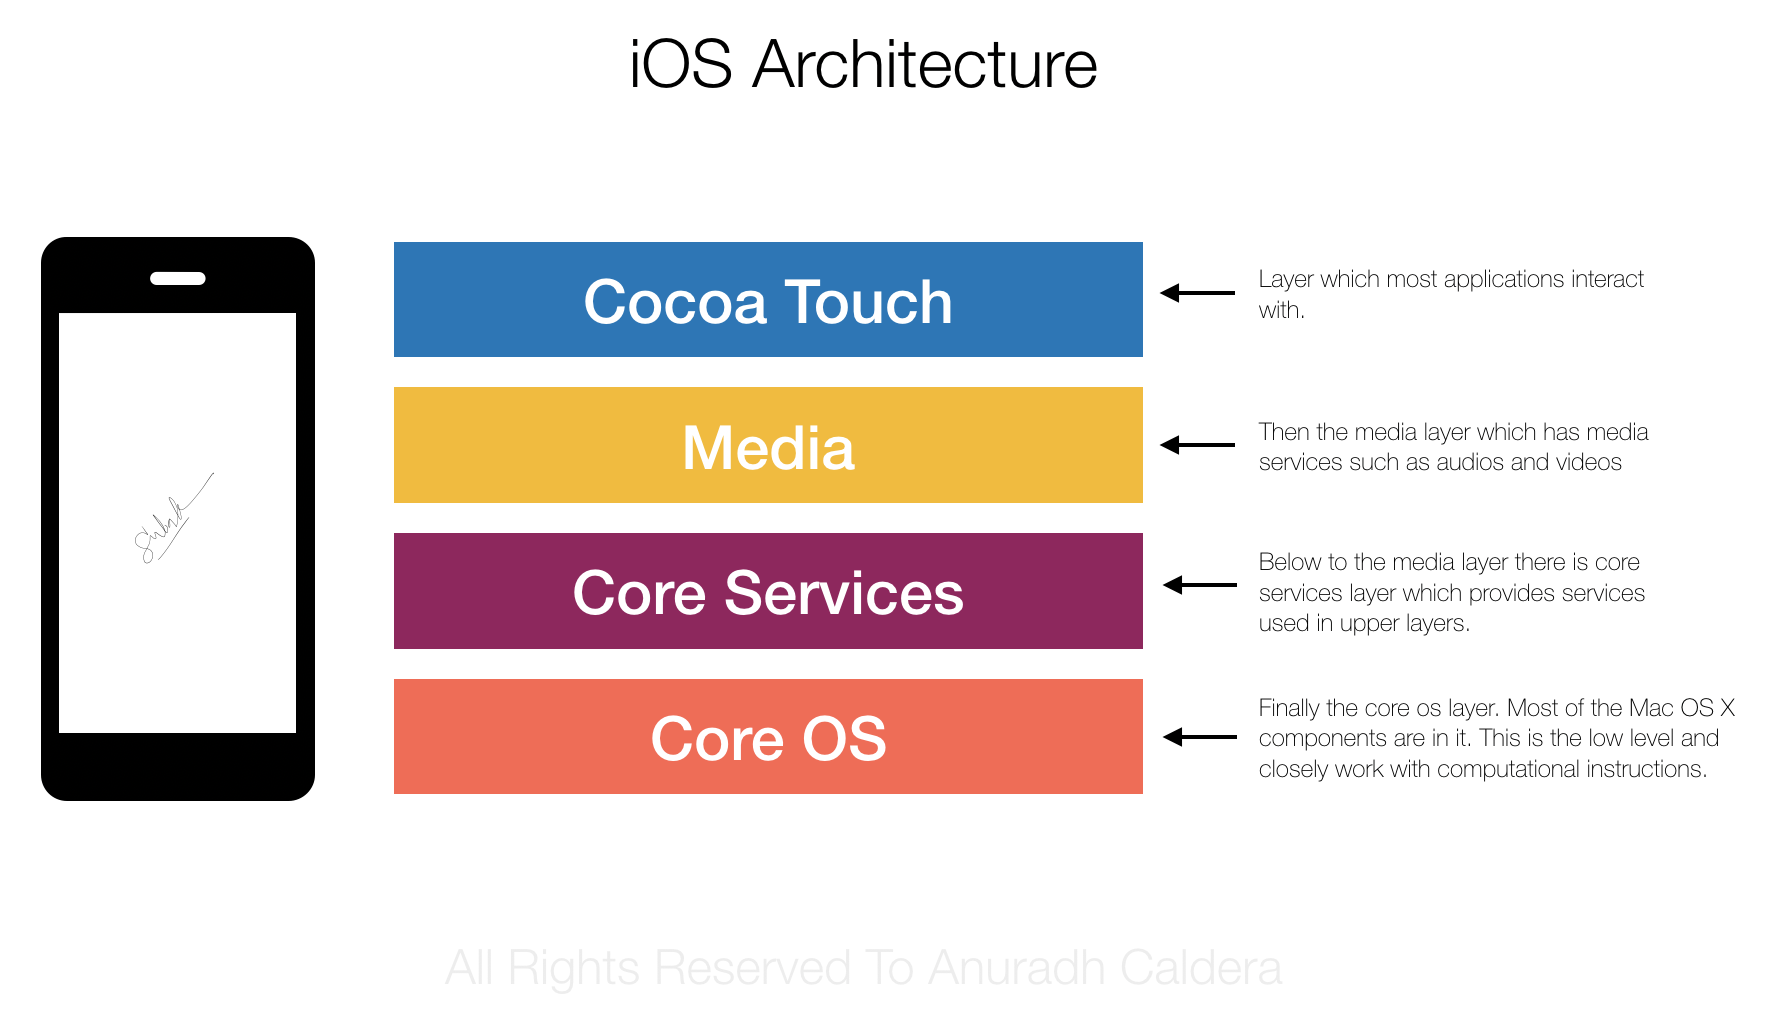
\includegraphics[width=6in]{images/Chapitre1/ios_architecture.png}
    \label{fig:ios Ui}
    \caption{L'architecture de iOS}
\end{figure}

\newpage
\section{Les applications mobiles}
\subsection{Definition}
Une application mobile est un logiciel installable sur les appareils mobile par exemple une tablette tactile ou un smartphone, pour but d'exécuter des tâches spécifiques.

La plupart des applications mobiles sont distribuées au public par le biais de plateformes de téléchargement généralement gérée par les fabricants de appareils mobiles comme Google Play Store par Android/Google ou encore App Store pour les produits Apple. Ces applications sont disponibles soit en version gratuite et qui contient généralement des publicités soit en version payante.

Sur certaines plateformes, les applications peuvent aussi être installées à partir de sources tierces, via un site non affilié au distributeur d'origine. Sur Android, cela est possible en activant le mode développeur. Sur iOS, cette manipulation est possible soit en étant développeur Apple, soit en possédant un appareil jailbreaké.~\cite{ApplicationMobile2020}

les applications mobiles se regroupent en plusieurs séries, on trouve : 
\begin{itemize}
   \item Les jeux mobiles.
   \item Les applications a but éducatif.
   \item Les applications de géolocalisation.
   \item Les applicatopns d'écoute de musiques ou de radios et de streaming vidéo.
   \item Les applications pour la consultation d'Internet.
   \item Les applications des réseaux sociaux.
\end{itemize}

\begin{figure}[!ht]
    \centering
    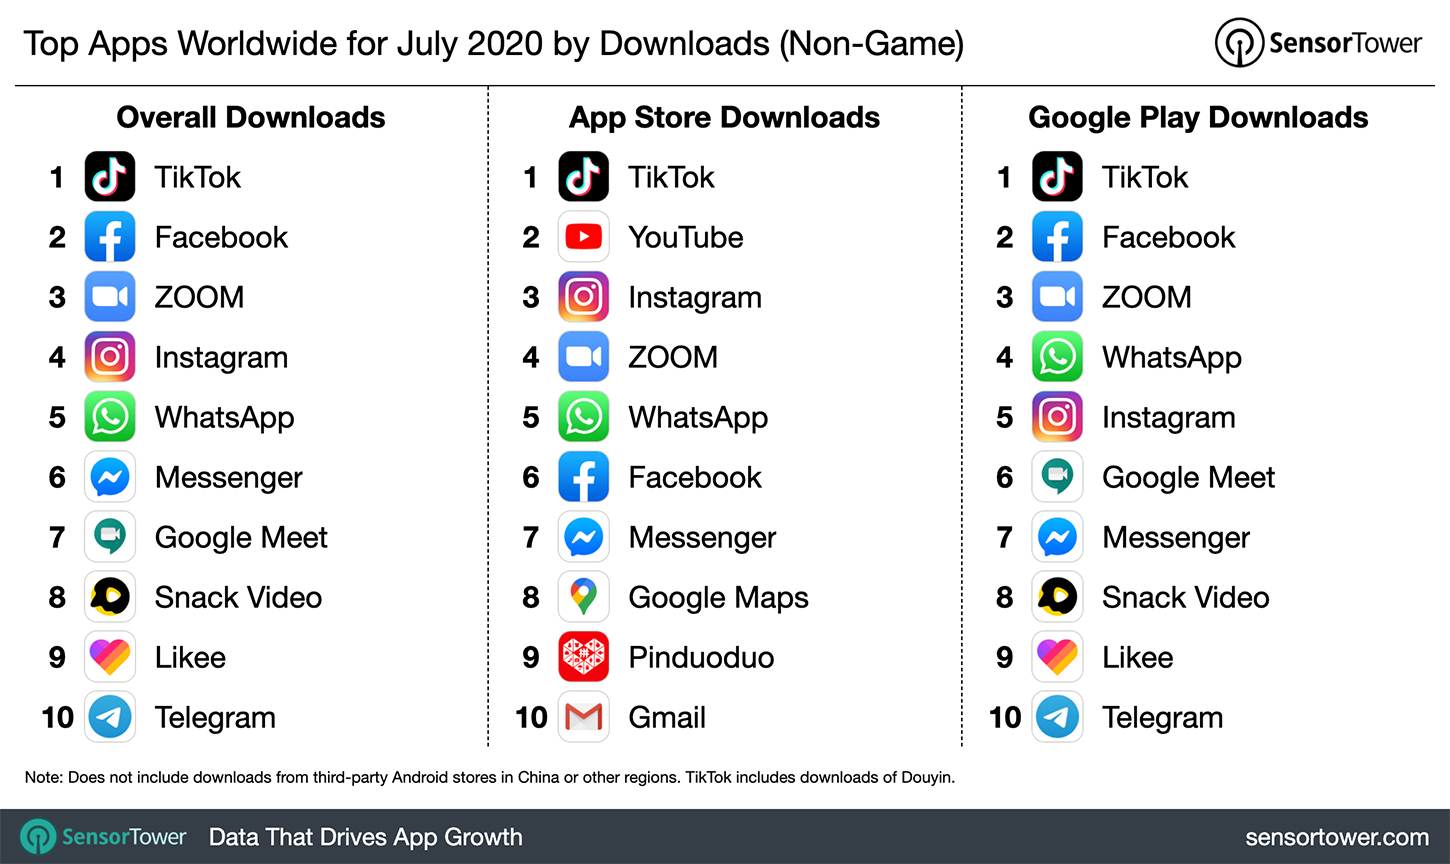
\includegraphics[width=4.6in]{images/Chapitre1/app_downloads.jpg}
    \label{fig:ios Ui}
    \caption{Classement des meilleures applications dans le monde pour juillet 2020 par téléchargements}
\end{figure}
\newpage
\subsection{Les types des applications mobiles}
Il existe dans le domaine des applications mobiles trois types d'applications en parlant du language de programmation et les taches que fait l'application. On trouve donc :
\subsubsection{Application native :}
Les applications natives sont des applications conçues spécialement pour les systèmes d'exploitation fiables par les smartphones. Ces applications utilisent chaqune un language de programmation spéciale pour chaque système d'exploitation, comme Java pour Android et Swift pour iOS.
\subsubsection{Application web :}
Une application web est une application conçue avec le language HTML et CSS, ce type d'application fonctionne de manière flexible sur tous les navigateurs internet dans les appareils mobiles. 
\subsubsection{Application hybride :}
Les applications hybrides regroupent les caractéristiques des applications web et applications mobilent, elles sont donc accessibles via toutes les plateformes des applications. ce type d'application réduit la durée et les charges du développement.


\begin{figure}[!ht]
    \centering
    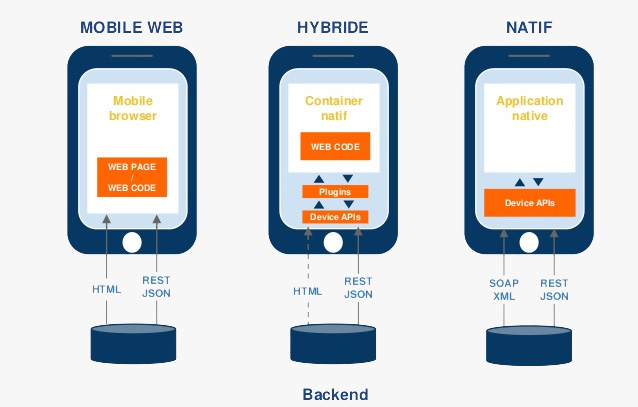
\includegraphics[width=6in]{images/Chapitre1/type_applications_mobile.jpg}
    \label{fig:type_applications}
    \caption{Les trois types d'applications mobile}
\end{figure}
\subsection{Le cycle de vie d'une application mobile}
Le cycle de vie d'une application mobile se compose de 6 phases de travail ~\cite{CycleVieDeveloppement}, citons-les:
     
\subsubsection{1- Planification et analyse:}
La première étape de la conception consiste à analyser la situation pour tenir compte des contraintes, des risques et de tout autre élément pertinent et assurer un ouvrage ou un processus répondant aux besoins du client.
\subsubsection{2- Spécification technique:}
Dans cette étape, On détermine le type des opérations ainsi que les systèmes pour lesquels on souhaite créer l'application mobile. On établit à la fin un cahier de charge.

\subsubsection{3- Prototypage et conception:}
À cette étape, des diagrammes UML ainsi que des diagrammes d'action sont créé puis on crée un prototype de l'application qui aide le client pour valider l'idée et commencer la phase suivante
\subsubsection{4- Développement:}
Le processus de développement d'applications est divisé en deux phases : front-end et backend. Cette étape consiste à coder les modules de l'application un par un et effectuer des tests sur place avant d'entamer le prochain module. Cependant, le développement de la partie backend n'est pas toujours nécessaire si on utilise des techniques cloud pour le traitement et le stockage des données 
\subsubsection{5- Tests et assurance de qualité:}
La phase de tests et assurance de qualité est une partie très importante pour la création de l'application. cette phase comprend des tests des exigences, interfaces et de la sécurité de l'application et des données ainsi que les ressources du bas niveau.
\subsubsection{6- Maintenance et mise à jour:}
Après la phase de tests,on est dans la phase finale où l'application est prête pour la distribution dans les plateformes d'achat des applications, mais le travail ne s'arrête pas là, l'application doit être mise à jour de façon reguiliére pour répondre aux nouveaux besoins des utilisateurs. 

